\documentclass{article}
\linespread{1.2}
\usepackage[margin = 1.25 in]{geometry}
\usepackage{wrapfig}
\usepackage{amsfonts}
\usepackage[utf8]{inputenc}
\usepackage[T1]{fontenc}
\usepackage{graphicx}
\usepackage[english]{babel}
\usepackage[algoruled]{algorithm2e}

\renewcommand{\theequation}{\thesection.arabic{equation}}

\renewcommand{\thefigure}{\thesection.\arabic{figure}}



\renewcommand{\vec}[1]{\mathbf{#1}}
\renewcommand{\theequation}{\thesubsection.\arabic{equation}}
\DeclareGraphicsExtensions{.pdf,.png,.jpg, .gif}

\usepackage{amsthm}

\usepackage[english]{babel}
\usepackage{mathtools}

%\usepackage[OT2,T1]{fontenc}
%\DeclareSymbolFont{cyrletters}{OT2}{wncyr}{m}{n}
%\DeclareMathSymbol{\sha}{\mathalpha}{cyrletters}{"58}

\DeclareFontFamily{U}{wncy}{}
\DeclareFontShape{U}{wncy}{m}{n}{<->wncyr10}{}
\DeclareSymbolFont{mcy}{U}{wncy}{m}{n}
\DeclareMathSymbol{\Sh}{\mathord}{mcy}{"58} 
\DeclareMathOperator*{\argmin}{arg\,min}

\newcounter{eqn}
\renewcommand*{\theeqn}{\alph{eqn})}
\newcommand{\num}{\refstepcounter{eqn}\text{\theeqn}\;}

\makeatother
\newcommand{\vectornorm}[1]{\left|\left|#1\right|\right|}
\newcommand*\conjugate[1]{\bar{#1}}

\newtheorem{thm}{Theorem}
\newtheorem{defn}{Definition}
 %\theoremstyle{plain}
  \newtheorem{theorem}{Theorem}[section]
  \newtheorem{corollary}[theorem]{Corollary}
  \newtheorem{proposition}[theorem]{Proposition}
  \newtheorem{lemma}[theorem]{Lemma}
\newtheorem{example}[theorem]{Example}
  \newtheorem{definition}[theorem]{Definition}
  \newtheorem{conj}[theorem]{Conjecture}
 \newtheorem{condition}{Condition}
 \newtheorem{remark}[theorem]{Remark}

\newcommand{\supp}{\operatorname{supp}} 
\newcommand{\vc}[1]{{\mathbf{ #1}}}
\newcommand{\tn}{\widetilde{\nabla}_{n} }
\newcommand{\Z}{{\mathbb{Z}}}
\newcommand{\re}{{\mathbb{R}}}
\newcommand{\II}{{\mathbb{I}}}
\newcommand{\ep}{{\mathbb{E}}}
\newcommand{\pr}{{\mathbb{P}}}
\newcommand{\FF}{{\mathcal{F}}}
\newcommand{\TT}{{\mathcal{T}}}
\newcommand{\phin}{\phig{n}}
\newcommand{\phig}[1]{\phi^{(#1)}}
\newcommand{\ol}[1]{\overline{#1}}
\newcommand{\eff}{{\rm eff}}
\newcommand{\suc}{{\rm suc}}
\newcommand{\tends}{\rightarrow \infty}
\newcommand{\setS}{{\mathcal{S}}}
\newcommand{\setP}{{\mathcal{P}}}
\newcommand{\setX}{{\mathcal{X}}}
\newcommand{\nec}{{\rm nec}}
\newcommand{\bd}{{\rm bd}}

\begin{document}
This is just a quick document for describing the differences between vanilla gradient descent, iterative thresholding and AMP.

\section{Gradient Descent}
Suppose we observe a vector \(y \in \re^m\), through an operator \(A \in \re^{m \times n}\), i.e. we have the model

\begin{equation}
y = Ax
\end{equation}

\(x \in \re^{n}\). One way to guess x, is to minimise the mean squared error:

\begin{equation}
J = \frac{1}{2}\vectornorm{y-Ax}_2^2 = \left(y-Ax\right)^T\left(y-Ax\right)
\end{equation}

We can do this by gradient descent, as 

\begin{equation}
\frac{\partial J}{\partial x} = A^T(y-Ax)
\end{equation}

So we have an iterative algorithm:

\begin{align*}
x^{t+1} = x^t + A^T(y-Ax^t)
\end{align*}

Putting it in a more suggestive form:

\begin{align*}
x^{t+1} &= x^t + A^Tz^t \\
z^t &= y - Ax^t
\end{align*}

\section{Iterative Thresholding}
The algorithm from the previous section will perform poorly, as we've not used any prior information about \(x\). We assume that \(x\) is sparse, so we now seek solutions to:

\begin{equation}
J = \frac{1}{2}\vectornorm{y-Ax}_2^2 + \lambda\vectornorm{x}_1
\end{equation}

The presence of the \(\ell_1\) norm, is inconvenient: \(J\) in this case has no formal gradient. In this case we can pretend that \(J\) is differentiable by doing a step in the direction of the gradient, and correcting for any error using the soft thresholding operator:\(S_\gamma\left(x\right)_i = \mathrm{sign}(x_i)\left(|x_i| - \gamma\right)^+\).

So our algorithm becomes:

\begin{align*}
x^{t+1} &= S_{\lambda}\left(x^t + A^Tz^t\right) \\
z^t &= y - Ax^t
\end{align*}

The soft-thresholding operator can be derived by considering the MAP estimate of the following model:

\begin{equation}
y = x + w
\end{equation}

where \(x\) is some (sparse) signal, and \(w\) is additive white Gaussian noise. We seek

\begin{equation}
\hat{x} = \arg\max_x \pr_{x|y}{\left(x|y\right)}
\end{equation}

This can be recast in the following form by using Bayes rule, noting that the denominator is independent of \(x\) and taking logarithms:

\begin{equation}
\hat{x} = \arg\max_x \left[\log{\pr_{w}{\left(y-x\right)}}+\log{\pr{\left(x\right)}}\right]
\label{hatx}
\end{equation}

The term \(\pr_{n}{\left(y-x\right)}\) arises because we are considering \(x+w\) with \(w\) zero mean Gaussian, with variance \(\sigma_n^2\). So, the conditional distribution of \(y\) (given \(x\)) will be a Gaussian centred at \(x\).

We will take \(\pr{\left(x\right)}\) to be a Laplacian distribution:

\begin{equation}
\pr{\left(x\right)} = \frac{1}{\sqrt{2}\sigma}\exp{-\frac{\sqrt{2}}{\sigma}|x|}
\end{equation}

Note that \( f\left(x\right) = \log{\pr_x{ \left( x \right)}} ~ -\frac{\sqrt{2}}{\sigma} |x| \), and so by differentiating \( f'\left(x\right) = -\frac{\sqrt{2}}{\sigma} \mathrm{sign}\left(x\right) \)

Taking the maximum of \ref{hatx} we obtain:

\begin{equation}
\frac{y-\hat{x}}{\sigma^2_n}-\frac{\sqrt{2}}{\sigma}sign(x) = 0
\end{equation}

Which leads the soft thresholding operation defined earlier, with \(\gamma = \frac{\sqrt{2}\sigma^2_n}{\sigma}\) as (via rearrangement):

$$
y =  \hat{x} + \frac{\sqrt{2}\sigma^2_n}{\sigma}\mathrm{sign}\left(x\right)
$$

or

$$
\hat{x}\left(y\right) = \mathrm{sign}(y)\left(y - \frac{\sqrt{2}\sigma^2_n}{\sigma}\right)_+
$$

i.e \(S_\gamma(y)\).

\section{AMP}
Approximate message passing further corrects this idea of pretending our optimisation objective is differentiable and correcting, by making a quadratic approximation to the likelihood of the model.

The algorithm becomes

\begin{align*}
x^{t+1} &= S_\lambda\left(x^t + A^Tz^t\right) \\
z^t &= y - Ax^t + b_tz^t
\end{align*}

which is similar to the iterative thresholding algorithm, but with an additional 'momentum' term added. A good choice of \(b\) is:

\begin{equation}
\frac{1}{m}\vectornorm{x^t}_0
\end{equation}

where \(\vectornorm{t}_0\) is the number of non-zero elements of t.

\section{DISTA}

\begin{figure}
\begin{algorithmic}[1]
\Procedure{DADMM}{$y_j,M_j,\varepsilon$}
\State $x^0 = 0$, $z^0 = 0$, $\theta^0 = 0$, $\eta^0 = 0$, \\  $Q =  \left(M_j^TM_j + (\rho D_J + 1) I\right)^{-1}$, $w_j = M_j^Ty_j $
\While{$\vectornorm{z^{k+1} - z^{k}} \leq \varepsilon$}
\For{$c = 1, \ldots, C}$
\State $x^{k+1} \gets Q\left(w_j+  z^k - \theta^{kT} -\nu^{kT}\right)$  
\State  $z^{k+1} \gets S_{\beta/\rho}\left(x_j^{k+1} \right) $  
\State $\theta^{k+1}\gets \theta_j^{k} + \rho \left(x^{k+1}-z^{k+1}\right)$  
\EndFor
\\Each node transmits $x^{k+1}$ in $\mathcal{N}_j$ and calculates
  \State $\nu_j^{k+1} \gets \nu_j^k + \rho\left(\sum_{m \in N_j} z_m^k - z_j^k\right)$
\EndWhile
\State \textbf{return} $z^{k+1}$
\EndProcedure
\end{algorithmic}
\caption{DADMM at Node \(j\)}\label{DADMM}
\end{figure}

\begin{figure}
\begin{algorithmic}[1]
\Procedure{DAMP}{$y_j,M_j,\varepsilon$}
\State $x^0 = 0$, $\alpha$, \\  \While{$\vectornorm{x_j^{k+1} - x_j^{k}} \leq \varepsilon$}
\\Each node transmits $x^{k}$ in $\mathcal{N}_j$ and calculates
  \State $x_j^{k+1/2} \gets \frac{1}{D_p+1)}\sum_{j \in N_j}x_j^{k}$
\For{$c = 1, \ldots, C}$
\State $x^{k+1} \gets x_j^{k+1/2} - \alpha S_{\beta}\left(M_j^Tx_j^{k+1/2} \right)$  
\EndFor

\EndWhile
\State \textbf{return} $x^{k+1}$
\EndProcedure
\end{algorithmic}
\caption{DAMP at Node \(j\)}\label{DAMP}
\end{figure}

\begin{figure}[h]
\centering
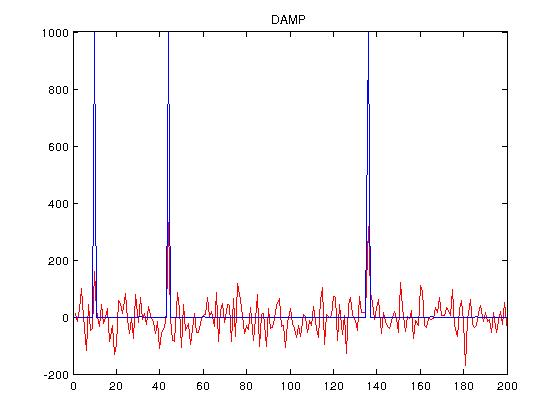
\includegraphics[height = 7.3 cm]{DAMP1000xhat.jpg}
\caption{DAMP estimate after 1000 iterations}
\label{fig:hvb}
\end{figure}

\begin{figure}[h]
\centering
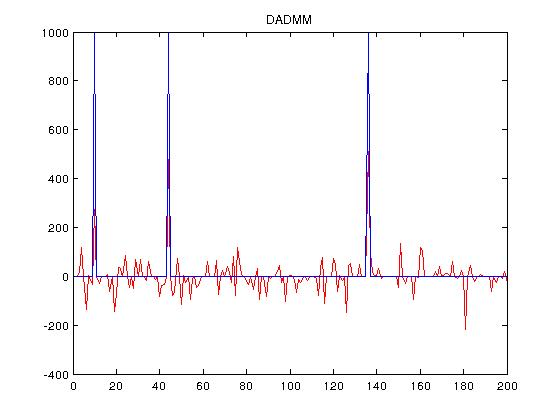
\includegraphics[height = 7.3 cm]{DADMM1000xhat.jpg}
\caption{DADMM estimate after 1000 iterations}
\label{fig:hvb}
\end{figure}

\begin{figure}[h]
\centering
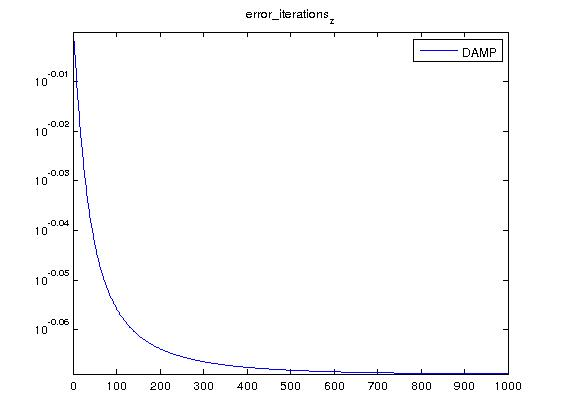
\includegraphics[height = 7.3 cm]{DAMP1000.jpg}
\caption{DAMP progress}
\label{fig:hvb}
\end{figure}

\begin{figure}[h]
\centering
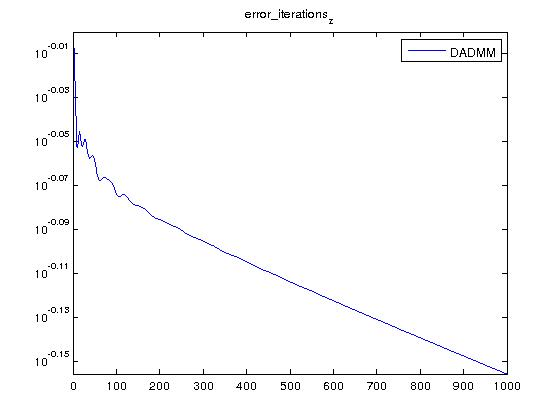
\includegraphics[height = 7.3 cm]{DADMM1000.jpg}
\caption{DADMM progress}
\label{fig:hvb}
\end{figure}

\begin{figure}[h]
\centering
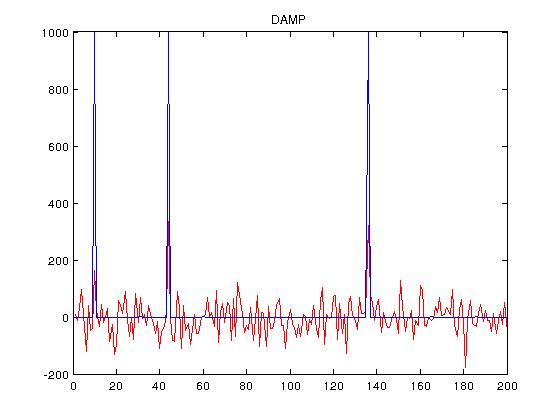
\includegraphics[height = 7.3 cm]{DAMPxhat5000.jpg}
\caption{DAMP estimate after 5000 iterations}
\label{fig:hvb}
\end{figure}

\begin{figure}[h]
\centering
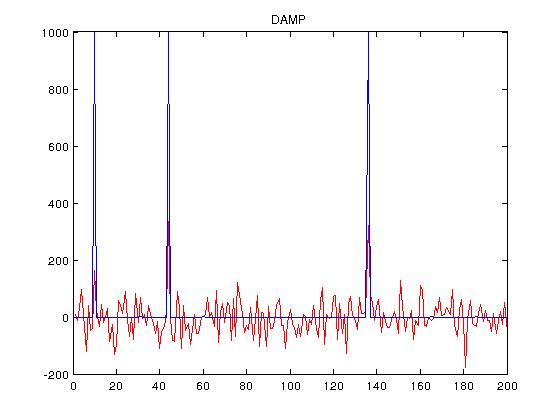
\includegraphics[height = 7.3 cm]{DADMMxhat5000.jpg}
\caption{DADMM estimate after 5000 iterations}
\label{fig:hvb}
\end{figure}

\begin{figure}[h]
\centering
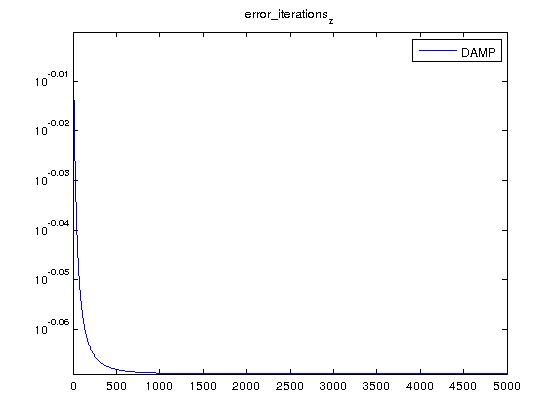
\includegraphics[height = 7.3 cm]{DAMP5000its.jpg}
\caption{DAMP progress}
\label{fig:hvb}
\end{figure}

\begin{figure}[h]
\centering
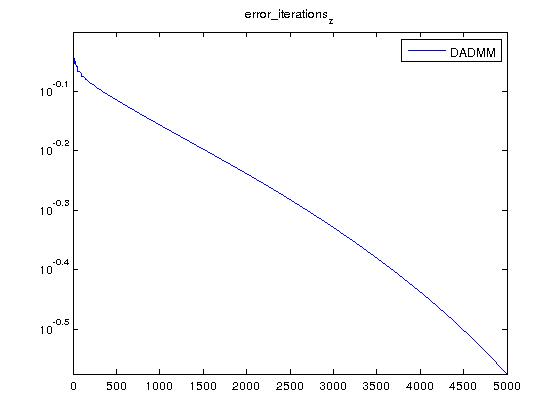
\includegraphics[height = 7.3 cm]{DADMM5000its.jpg}
\caption{DADMM progress}
\label{fig:hvb}
\end{figure}


\end{document}

